\documentclass[english, a4paper, 12pt]{report}

% Overall document aspect
\usepackage[utf8]{inputenc}
\usepackage[english]{babel}
\usepackage[toc,page]{appendix}
\usepackage[skip=0.75\baselineskip plus 2pt]{parskip}
\usepackage{geometry}
\geometry{vmargin=2.5cm}
\usepackage{changepage}
\usepackage{adjustbox}

% For specific parts, tools
\usepackage{hyperref}
\usepackage[toc,page]{appendix}
\usepackage{enumitem}

% Tables
\usepackage{tabularray}
\usepackage{pifont}
\usepackage{xcolor}
\usepackage{breqn}
\usepackage{booktabs}
\newcommand{\cmark}{\textcolor{green!80!black}{\ding{51}}}
\newcommand{\xmark}{\textcolor{red}{\ding{55}}}
\usepackage{multirow}

% For images
\usepackage{graphicx}
\usepackage[skip=0.5\baselineskip]{caption}
\usepackage{subcaption}
\usepackage{wrapfig}
\usepackage{tikz}
\usepackage{float} % For forcing placement

% Maths
\usepackage{amsmath}
\usepackage{amsfonts}
\usepackage{amsthm}
\usepackage{amssymb}
\usepackage{mathtools}
\usepackage{bbm}

\newtheorem{theorem}{Theorem}[section]
\newtheorem{proposition}{Proposition}[theorem]
\newtheorem{corollary}{Corollary}[theorem]
\newtheorem{lemma}[theorem]{Lemma}


\hypersetup{
colorlinks=true,
linkcolor=purple,
citecolor=purple,
filecolor=magenta,      
urlcolor=cyan,
pdfpagemode=FullScreen,
}



% Citing code
\usepackage{listings}

\renewcommand{\ttdefault}{cmtt}
\DeclareFixedFont{\ttb}{T1}{cmtt}{bx}{n}{12} % for bold
\DeclareFixedFont{\ttm}{T1}{cmtt}{m}{n}{12}  % for normal
% Custom colors
\usepackage{color}
\definecolor{deepblue}{rgb}{0,0,0.5}
\definecolor{deepred}{rgb}{0.6,0,0}
\definecolor{deepgreen}{rgb}{0,0.5,0}
% Python style for highlighting
\newcommand\pythonstyle{\lstset{
language=Python,
basicstyle=\ttm,
morekeywords={self},              % Add keywords here
keywordstyle=\ttb\color{deepblue},
emph={MyClass,__init__},          % Custom highlighting
emphstyle=\ttb\color{deepred},    % Custom highlighting style
stringstyle=\color{deepgreen},
frame=tb,                         % Any extra options here
showstringspaces=false
}}
\newcommand\pythoninline[1]{{\pythonstyle\lstinline!#1!}}
%====================== PACKAGES ======================

\usepackage[english]{babel}
\usepackage[utf8x]{inputenc}

% General document layout
\usepackage{abstract}
\usepackage[style=verbose-ibid,backend=bibtex]{biblatex}
\usepackage{hyperref}
\usepackage{tcolorbox}
\usepackage{setspace}
% Margins
\usepackage[T1]{fontenc}
\usepackage[top=2cm, bottom=2cm, left=2cm, right=2cm]{geometry}

% Scientific writing
\usepackage{amsmath}
\usepackage{amssymb}
\usepackage{bbm}
\usepackage{mathtools}

% Tikz illustrations
\usepackage{graphicx}
\usepackage{float}
\usepackage{tikz}
\usepackage{pgfplots}
\pgfplotsset{compat=1.18}

% Bibliography stuff
\usepackage[
backend=biber,
style=alphabetic,
sorting=ynt,
natbib=true
]{biblatex}

\addbibresource{biblio.bib}

%==== INFORMATION ET REGLES ======================

% Numbering
\setcounter{secnumdepth}{3}
\setcounter{tocdepth}{3}

\hypersetup{
pdfauthor = {Vivien Tisserand},
pdftitle = {Quantitative finance\\ Interviews preparation \& a bunch of other things},
}

%======================== DOCUMENT ========================

\begin{document}

% Line spacing
\newcommand{\HRule}{\rule{\linewidth}{0.5mm}}

\begin{titlepage}
   \begin{center}
       \vspace*{1cm}

        \Large
       \textbf{Quantitative finance}

        \large
       \vspace{0.5cm}
        Interviews preparation
            
       \vspace{1.5cm}

       \textbf{Vivien Tisserand}

       \vfill
            
       \vspace{0.8cm}
     

    \textbf{Abstract}
    \end{center}
    
    This is a summary of interview questions found on the internet, books, \textit{etc.}, along with more in-depth digressions related to quantitative finance. It is a mixed of applied mathematics and computer science.\\
    I am not found of brainteasers, they are a poor way to assess for a candidate's ability to be an asset for the team. This work smoothly transitioned to a sort of \textit{vademecum} in applied mathematics: through several questions, it goes through different techniques that are easy to forget with time. I myself refer to it quite often when I forget about how to write the Lagrangian in a constrained optimization problem, or the general solution of a second-order differential equation...
    
\end{titlepage}


\tableofcontents
\thispagestyle{empty}
\setcounter{page}{0}

\chapter{Probability}

\section{Correlated bivariate distribution}

\begin{tcolorbox}[width=\linewidth, sharp corners=all, colback=white!95!black]
Let $(X,Y)$ follow a bivariate normal standard distribution with correlation $\rho$. Find the expectation: $$\mathbb{E}[\operatorname{sgn}(X)\operatorname{sgn}(Y)].$$
\end{tcolorbox}

We are interested in the joint distribution of $X$ and $Y$:
$$\begin{pmatrix}X\\Y\end{pmatrix} \sim \mathcal{N}\left(\begin{pmatrix}0\\0\end{pmatrix}, \begin{pmatrix}
1 & \rho\\ \rho & 1
\end{pmatrix}\right).$$

To see what happens here, we can compare the density contour of this distribution with the independent case. The covariance matrix is symmetric thus diagonalizable. We can find its eigenvalues and its eigenvectors (through classic computations or noticing this is a circulant matrix). With $P = \begin{pmatrix}
1 & 1\\ 1 & -1
\end{pmatrix}$,
$$\Sigma = P\begin{pmatrix}
1+\rho & 0\\ 0 & 1-\rho
\end{pmatrix}P^{-1}.$$
This gives us the shape of the correlated distribution. Qualitatively, we can say that, as $\rho$ defines how rotated and squished the distribution is, the bigger $\rho$, the higher the probabiliy of $X$ and $Y$ being the same sign.

\begin{figure}[H]
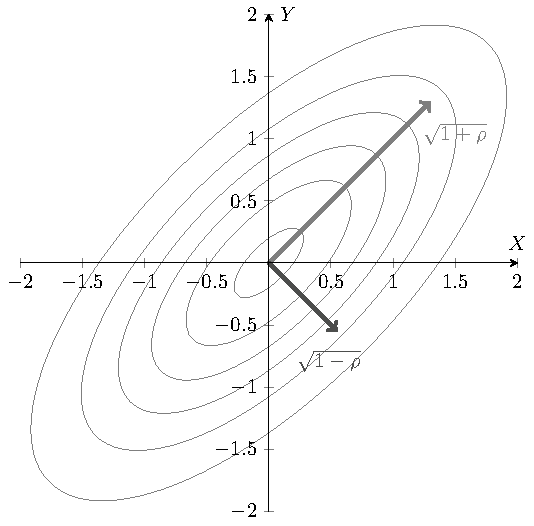
\includegraphics[width=0.35\textwidth]{img/tikz/bivariate_contour.pdf}
\centering
\caption{Density contours of a bivariate normal law, with $\rho=0.7$}
\label{fig:bivariate_contour}
\end{figure}


Back to our problem: the random variable $\operatorname{sgn}(X)\operatorname{sgn}(Y)$ takes values in the set $\{-1,1\}$. Thus, to get its expectancy, we can compute these discrete probabilities:
\begin{align*}
    \mathbb{E}[\operatorname{sgn}(X)\operatorname{sgn}(Y)] &= 1\times \mathbb{P}(\operatorname{sgn}(X)\operatorname{sgn}(Y)=1) -1\times \mathbb{P}(\operatorname{sgn}(X)\operatorname{sgn}(Y)=-1)\\
    &= 1\times \mathbb{P}(\operatorname{sgn}(X)\operatorname{sgn}(Y)=1) -1\times (1-\mathbb{P}(\operatorname{sgn}(X)\operatorname{sgn}(Y)=1))\\
    &= 2\mathbb{P}(\operatorname{sgn}(X)\operatorname{sgn}(Y)=1) -1.
\end{align*}

Using the symmetry of the distribution, $$\mathbb{P}(\operatorname{sgn}(X)\operatorname{sgn}(Y)=1) = \mathbb{P}(X>0,Y>0) + \mathbb{P}(X<0,Y<0) = 2\mathbb{P}(X>0,Y>0),$$

thus the only thing we need to compute is $\mathbb{P}(X>0,Y>0)$.\\

If $$\begin{pmatrix}U\\V\end{pmatrix} = \Sigma^{-1/2}\begin{pmatrix}X\\Y\end{pmatrix},$$
then $(U,V)$ follows an independent bivariate normal standard distribution. Inverting $\Sigma$ we get:
$$\Sigma^{-1} = \frac1{1-\rho^2}\begin{pmatrix}
1 & -\rho\\ -\rho & 1
\end{pmatrix}.$$

\begin{figure}[H]
    \centering
    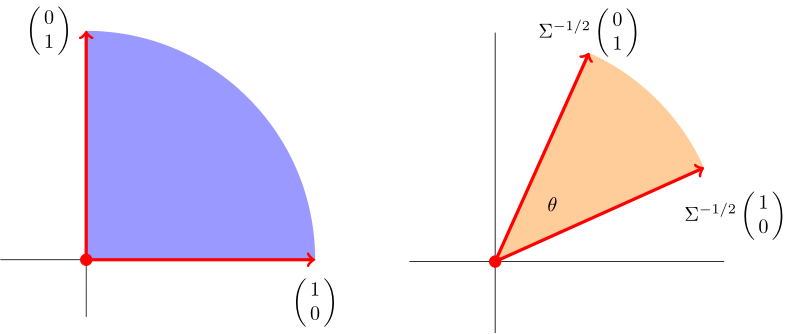
\includegraphics[width=0.8\textwidth]{img/corr_biv_normal.png}
    \caption{Area of the event $X>0,Y>0$ for $\rho = 0$ (left) and $\rho \ne 0$ (right). From \href{https://math.stackexchange.com/questions/1687795/correlated-joint-normal-distribution-calculating-a-probability}{here}.}
\end{figure}

Then, there exists a $\theta \in [0,2\pi]$ such that $\mathbb{P}(X>0,Y>0) = \dfrac{\theta}{2\pi}$. This $\theta$ verifies $$\cos{\theta} = \dfrac{\langle u,v\rangle}{\|u\| \|v\|}.$$ with $u = \Sigma^{-1/2} \begin{pmatrix}1\\0\end{pmatrix}$ and $v = \Sigma^{-1/2} \begin{pmatrix}0\\1\end{pmatrix}$


$$\langle u,v\rangle = (1\ 0)\,\Sigma^{-1}(0\ 1)^T=-\rho/(1-\rho^2)$$
$$\|u\|^2=(1\ 0)\,\Sigma^{-1}(1\ 0)^T=1/(1-\rho^2)$$
$$\|v\|^2=(0\ 1)\,\Sigma^{-1}(0\ 1)^T=1/(1-\rho^2)$$

so that $\cos(\theta)=-\rho.$ Putting it all together gives 
$$\mathbb{P}(X>0,Y>0)=\dfrac{\arccos(-\rho)}{ 2\pi}.$$

Finally, $$\boxed{ \mathbb{E}[\operatorname{sgn}(X)\operatorname{sgn}(Y)] = \dfrac{2\arccos(-\rho)}{\pi} - 1. }$$

Note that if $\rho=0$, we have $\mathbb{E}[\operatorname{sgn}(X)\operatorname{sgn}(Y)]=0$ ; it converges to $1$ as $\rho \longrightarrow 1$ and to $-1$ as $\rho \longrightarrow -1$, which gives us confidence in our answer.

\section{The coupons collector}

\begin{tcolorbox}[width=\linewidth, sharp corners=all, colback=white!95!black]
A chocolate company launches a marketing campaign: for each chocolate bar you buy, you get one collectible card out of a set of $n$ possible cards. We can assume the card are uniformly distributed among the chocolate bars.\newline
How many chocolate bars should you buy to complete the collection?
\end{tcolorbox}

Well, at least $n$, even if we are very lucky.\newline
The first bar we open will yield to a new card. For the second bar, we have a probability $\dfrac{1}{n}$ to get the same card we already have, thus $\dfrac{n-1}{n}$ to get a new card. This follows a geometric law: the expectation for such an event is $\dfrac{n}{n-1}$. And so on, decreasing the probability for each new card we acquire.\newline
The total expectancy will be the sum of all of these individual processes: 
$$\mathbb{E}\left[ N \right] = \displaystyle \sum_{k=0}^{n-1} \dfrac{n}{n-k},$$
with N the random variable that counts the number of chocolate bars eaten to get the full collection.\\

We realize that we are actually dealing with the harmonic sum $H_n = \sum_{k=1}^{n} \frac1{k}$, which can be squeezed between two integrals to get the equivalent: $H_n \sim_{n \to +\infty} \log(n).$\newline
Thus $N \sim_{n \to +\infty} n\log(n).$\\

To give a confidence interval around the number of chocolate bars we should buy, let's pull up some concentration inequalities.\newline
We still deal with the sum of independent geometric variables so the variance is easy to compute:

\begin{align*}
    \operatorname{Var}[N] &= \displaystyle \sum_{k=1}^n \operatorname{Var}[N_i]\\
    &= \displaystyle \sum_{k=1}^n \left(1 - \dfrac{n-k+1}{n}\right)\left(\dfrac{n}{n-k+1}\right)^2\\
    &= n\displaystyle \sum_{k=1}^n \dfrac{k-1}{(n-k+1)^2} \sim_{n \to +\infty} n \dfrac{\pi^2}{6}. 
\end{align*}

Applying Chebychev's inequality, we get: $$\mathbb{P}(\lvert \mathbb{E}[N] - N \rvert \geq k \sigma) \leq \dfrac{1}{k^2}.$$

Some other inequalities could be used to raffinate this result: Chernoff bounds, Vysochanskij–Petunin inequality, etc.




\chapter{Statistics}

\section{Estimating the support of an uniform law}

\begin{tcolorbox}[width=\linewidth, sharp corners=all, colback=white!95!black]
Suppose that we have $x_1,\dots,x_n$ observations from an uniform law $X \sim \mathcal{U}[0,\theta]$, where $\theta$ is an unknown parameter that we want to estimate. Give at least two estimators for $\theta$ and compare them.
\end{tcolorbox}

\paragraph*{Method of moments:}\\

Having a look at the first order moment, it appears that $\mathbb{E}[X] = \theta/2$. Taking the empirical counter-party of this theoretical quantity, we have $\boxed{\hat{\theta}^{\text{MM}} = \dfrac{2}{n}\sum\limits_{i=1}^n x_i.}$\newline
By applying the strong law of large numbers and the continuous mapping theorem, $\hat{\theta}^{\text{MM}} \xrightarrow{a.s.} \theta$. Thus \boxed{\text{this estimator is consistent}}.\newline
We want asymptotic results on the convergence of this estimator. Before using the CLT, we have to check for the existence of a second-order moment.

\begin{align*}
    \mathbb{E}[X^2] &= \displaystyle \int_{\mathbb{R}} x^2 f(x) \, \mathrm{d}x \\
    &= \displaystyle \int_{0}^{\theta} x^2 \dfrac{1}{\theta} \, \mathrm{d}x \\
    &= \left[ \dfrac{1}{3\theta}x^3 \right]^\theta_0 \\
    &= \dfrac{\theta^2}{3} < +\infty
\end{align*}

Thus, we have $\mathbb{V}[X] = \mathbb{E}[X^2] - \mathbb{E}[X]^2 = \dfrac{\theta^2}{12}$. So, $\mathbb{V}[2X_1]  = \dfrac{\theta^2}{3}$.\newline

By applying the central limit theorem, we have : $$\sqrt{n}(\hat{\theta}^{\text{MM}} - \theta) \xrightarrow{(d)} \mathcal{N}\left(0, \dfrac{\theta^2}{3}\right).$$

We have to evaluate the risk of this estimator, that we write as the sum of the squared bias and the variance : $$\text{MSE}(\hat{\theta}^{\text{MM}}) = \mathbb{E}[(\hat{\theta}^{\text{MM}} - \theta)^2] = \mathbb{E}[(\hat{\theta}^{\text{MM}} - \mathbb{E}[\hat{\theta}^{\text{MM}}])^2] + \mathbb{E}[\hat{\theta}^{\text{MM}} - \theta]^2 = \mathbb{V}[\hat{\theta}^{\text{MM}}] + (\mathbb{E}[\hat{\theta}^{\text{MM}}] - \theta)^2.$$

We have $\mathbb{E}[\hat{\theta}^{\text{MM}}] = 0$ and $\mathbb{V}[\hat{\theta}^{\text{MM}}] = \dfrac{1}{n^2}n\mathbb{V}[2X_1] = \dfrac{\theta^2}{3n}.$\newline

Thus, $$\text{MSE}(\hat{\theta}^{\text{MM}}) = \dfrac{\theta^2}{3n}.$$


\paragraph*{Maximum likelihood:}

Let's write the likelihood of this model:

\begin{align*}
    L((X_1,\dots,X_n), \theta) &= \displaystyle \prod_{i=1}^{n} f_X(X_i) \\
    &= \displaystyle \prod_{i=1}^{n} \dfrac{1}{\theta} \mathbbm{1}_{[0, \theta]}(X_i)\\
    &= \dfrac{1}{\theta^n} \prod_{i=1}^{n} \mathbbm{1}_{[0, \theta]}(X_i).
\end{align*}

And this function is maximized by choosing the smallest $\theta$ such that all of the $X_i$ lie in $[0, \theta]$, that is $\hat{\theta}^{\text{MLE}} = \max_{1\leq i \leq n} X_i.$\newline

To check the consistency of this estimator, we will have a look at its convergence (in probability). Let $\theta \in \Theta$ and $\varepsilon >0$ :

\begin{align*}
    \mathbb{P}_\theta(\lvert\hat{\theta}^{\text{MLE}} - \theta\rvert \ge \varepsilon) &= \mathbb{P}_\theta(\hat{\theta}^{\text{MLE}} \ge \theta + \varepsilon) + \mathbb{P}_\theta(\hat{\theta}^{\text{MLE}} \le \theta - \varepsilon)\\
    &= 0 + \mathbb{P}_\theta(\max_{1\leq i \leq n} X_i \le \theta - \varepsilon)\\
    &= \prod_{i=1}^{n} \mathbb{P}_\theta(X_i \le \theta - \varepsilon)\\
    &= \left(1 - \dfrac{\varepsilon}{\theta} \right)^n \underset{n\to +\infty}{\longrightarrow} 0.
\end{align*}


Thus, $\hat{\theta}^{\text{MLE}} \xrightarrow{\mathbb{P}} \theta$ : this estimator is consistent.\newline

In order to estimate the risk of this estimator, we have to look at the law that the maximum of $n$ independent uniform laws follows. This is done by looking at the cumulative distribution function. Let $x \in [0,\theta] :$

\begin{align*}
    \mathbb{P}_\theta(X_{(n)} \le x) &= \mathbb{P}_\theta\left(\bigcap_{i=1}^{n} {X_i \le x}\right)\\
    &= \prod_{i=1}^{n} \mathbb{P}_\theta(X_i \le x)\\
    &= \left(\dfrac{x}{\theta}\right)^n.
\end{align*}

Thus, $$F_{X_{(n)}} = \begin{cases}
        0 & \text{if } x < 0\\
        \left(\dfrac{x}{\theta}\right)^n & \text{if } 0 \le x \le \theta\\
        1 & \text{if } x>\theta
        \end{cases}$$

This cdf as smooth as we need to take its derivative: that will be the density we were looking for:

$$f_{X_{(n)}}(x) = n \dfrac{x^{n-1}}{\theta^n} \mathbbm{1}_{[0, \theta]}(x)$$

Let's compute the bias and the variance.\newline

$$\mathbb{E}[\hat{\theta}^{\text{MLE}}] = \displaystyle \int_{\mathbb{R}} x f_{X_{(n)}}(x) \, \mathrm{d}x = \displaystyle \int_{0}^{\theta} \dfrac{n}{\theta^n} x^n \, \mathrm{d}x = \dfrac{n}{\theta^n} \left[ \dfrac{x^{n+1}}{n+1}\right]^\theta_0 = \dfrac{n}{n+1}\theta.$$

Then, the bias is : $B(\hat{\theta}^{\text{MLE}}) = \dfrac{n}{n+1}\theta - \theta = -\dfrac{1}{n+1}\theta \ne 0.$ We can introduce a corrected estimator that we will consider too : $\hat{\theta}_{\text{corr}}^{\text{MLE}} = \dfrac{n+1}{n} \hat{\theta}^{\text{MLE}}$, such that $\mathbb{E}[\hat{\theta}_{\text{corr}}^{\text{MLE}}] = \theta$:  an unbiased estimator.\newline

Then, we have $$\mathbb{E}[(\hat{\theta}^{\text{MLE}})^2] = \displaystyle \int_{\mathbb{R}} x^2 f_{X_{(n)}}(x) \, \mathrm{d}x = \displaystyle \int_{0}^{\theta} \dfrac{n}{\theta^n} x^{n+1} \, \mathrm{d}x = \dfrac{n}{\theta^n} \left[ \dfrac{x^{n+2}}{n+2}\right]^\theta_0 = \dfrac{n}{n+2}\theta^2.$$ And $$\text{MSE}(\hat{\theta}^{\text{MLE}}) = \mathbb{E}[(\hat{\theta}^{\text{MLE}} - \theta)^2] = \mathbb{E}[(\hat{\theta}^{\text{MLE}})^2] -2 \theta \mathbb{E}[\hat{\theta}^{\text{MLE}}] + \theta^2$$

Thus, $$\text{MSE}(\hat{\theta}^{\text{MLE}}) = \dfrac{n}{n+2}\theta^2 - 2\dfrac{n}{n+1}\theta^2 + \theta^2 = \dfrac{2\theta^2}{(n+1)(n+2)}.$$

And $$\text{MSE}(\hat{\theta}_{\text{corr}}^{\text{MLE}}) = \left(\dfrac{n+1}{n}\right)^2 \mathbb{E}[(\hat{\theta}^{\text{MLE}})^2] - 2\dfrac{n+1}{n}\theta \mathbb{E}[(\hat{\theta}^{\text{MLE}} + \theta^2 = \dfrac{\theta^2}{n(n+1)}.$$

\paragraph*{Maximum a posteriori:}

We write the likelihood of the model in terms of $\theta$ :
$$L((X_1,\dots,X_n), \theta) = \dfrac{1}{\theta^n} \prod_{i=1}^{n} \mathbbm{1}_{[0, \theta]}(X_i) = \dfrac{1}{\theta^n} \mathbbm{1}_{[X_{(n)}, =\infty[}(\theta).$$

\textbf{Remark :} the set such that $L(., \theta)>0$ is $[0, \theta]$ : it depends on $\theta$, thus the model is not regular. Keep that in mind when dealing with Fisher information for instance.\newline

\begin{enumerate}
    \item \textbf{Flat prior:}\newline

We apply the definition for a Bayesian estimator with a prior density $\pi_0$ :

\begin{align*}
    \hat{\theta}^{\text{B}} &= \dfrac{\displaystyle \int_{\Theta} \theta L(x, \theta) \pi_0(\theta) \, \mathrm{d}\lambda(\theta)}{\displaystyle \int_{\Theta} L(x, \theta) \pi_0(\theta) \, \mathrm{d}\lambda(\theta)}\\
    &= \dfrac{\displaystyle \int_{X_{(n)}}^{+\infty} \theta^{-n+1} \, \mathrm{d}\theta}{\displaystyle \int_{X_{(n)}}^{+\infty} \theta^{-n} \, \mathrm{d}\theta}\\
    &= \dfrac{n-1}{n-2}X_{(n)}.
\end{align*}

Bias and MSE are not computed there for sanity reasons.

    \item \textbf{Jeffreys prior:}\newline

The density function of this prior is proportional to the squareroot of the determinant of the Fisher information matrix.\newline

Thus we need to compute this quantity for this model, with n observations (as it is not regular, $I_n \ne n I_1$) :

$$I_n(\theta) = \mathbb{E}\left[\dfrac{\partial \log L_n(\theta)}{\partial \theta}^2\right]$$

We have $I_n(\theta) = \mathbb{E}[(-n/\theta)^2] = \dfrac{n^2}{\theta^2}$\newline

(If we had taken the expectancy of the second-order derivative of the log-likelihood, we would not have had the same result has the model is not regular.)\newline

This gives us the noninformative prior (Jeffreys) : $\pi_0(\theta) \propto \theta^{-1}.$


\end{enumerate}





\section{Building a statistical test}

\begin{tcolorbox}[width=\linewidth, sharp corners=all, colback=white!95!black]
Let's assume you have a batch of a hundred observations (numbers). There are two hypotheses and one is true :
\begin{itemize}
    \item $H_0$: these observations are independent draws from a Gaussian $\mathcal{N}(0, 1/18)$,
    \item $H_1$:  each observation has been obtained by averaging $6$ uniforms $\mathcal{U}([-1,1])$ random variables.
\end{itemize}
How would you find out which scenario is true.\\

\textit{Taken from @adad8m on Twitter.}
\end{tcolorbox}


\chapter{Machine learning}

\section{Linear regression}

\begin{tcolorbox}[width=\linewidth, sharp corners=all, colback=white!95!black]
We are interested in the basic linear regression model where given observations $(x_i, y_i)_{1\leq i \leq n}$ we want to build the model $$Y = \alpha + \beta X + \varepsilon.$$

Explain the underlying assumptions in the model and derive estimators for the coefficients.

\end{tcolorbox}

The underlying assumptions of the linear model are the following:

\begin{itemize}
    \item No perfect multicollinearity between the explanatory variables, otherwise the parameter $\beta$ is not identifiable. This is the \textbf{full-rank} assumption.
    \item Independence of errors. Generalized least squares can handle correlated errors.
    \item \textbf{Homoscedasticity}, or constant variance, which can be tested on the residuals. If there is heteroscedasticity, the Gauss-Markov theorem doesn't apply, thus the estimators derived are not the Best Linear Unbiased Estimators (BLUE). It can be corrected thanks to a weighted least squares approach, or a logarithmization of the data.
    \item \textbf{Exogeneity}.
\end{itemize}

We have to minimize the Euclidean distance between the predicted values by the model for $Y$, $\hat{Y}$ and the actual values. This can be written as :
$$(\hat{\alpha}, \hat{\beta}) \in \operatorname{argmin}_{(\alpha, \beta) \in \mathbb{R}^2} \displaystyle \sum_{i=1}^{n} (y_i - \hat{y_i})^2$$

Replacing with the model, we have to find parameters that minimize $f(\alpha, \beta) = \displaystyle \sum_{i=1}^{n} (y_i - (\alpha + \beta x_i))^2.$ We will write the first order conditions and check by computing the Hessian that we are actually looking at a minimum.

$$\left\{\begin{array}{ll}
        \dfrac{\partial f}{\partial \alpha}(\alpha, \beta) &= 0 \\
        \dfrac{\partial f}{\partial \beta}(\alpha, \beta) &= 0
    \end{array}\right. \Leftrightarrow 
\left\{\begin{array}{ll}
        -2\sum_i (y_i - \alpha - \beta x_i) &= 0 \\
        -2\sum_i x_i (y_i - \alpha - \beta x_i) &= 0
    \end{array}\right.$$

The first line give $\hat{\alpha} = \overline{y} - \hat{\beta} \overline{x}$ while the second line can be written as the following : 
\begin{equation*}
\begin{aligned}
    \sum_i x_i (y_i - \hat{\alpha} - \hat{\beta} x_i) &= \sum_i y_i x_i - (\overline{y} - \hat{\beta} \overline{x})x_i - \hat{\beta} x_i^2\\
    &= \sum_i y_i - \overline{y} + \hat{\beta} (\overline{x} - x_i).
\end{aligned}
\end{equation*}

Thus 
\begin{equation*}
\begin{aligned}
    &\sum_i x_i (y_i - \hat{\alpha} - \hat{\beta} x_i) = 0 &\Leftrightarrow \sum_i y_i - \overline{y} + \hat{\beta} (\overline{x} - x_i) = 0\\
    &\Leftrightarrow \hat{\beta} = \dfrac{\sum_i y_i - \overline{y}}{\sum_i x_i - \overline{x}}\\
    &\Leftrightarrow \hat{\beta} = \dfrac{\sum_i (y_i - \overline{y})(x_i-\overline{x})}{\sum_i (x_i - \overline{x})^2}\\
    &\Leftrightarrow \boxed{\hat{\beta} = \dfrac{\widehat{\operatorname{Cov}}(X, Y)}{\widehat{\operatorname{Var}}(X)}.}
\end{aligned}
\end{equation*}





\chapter{Financial mathematics}

\section{Dupire formula for local volatility}

\begin{tcolorbox}[width=\linewidth, sharp corners=all, colback=white!95!black]
Explain the motivation behind local volatility and prove Dupire formula.
\end{tcolorbox}

The Black-Scholes model is really convenient as it has few parameters, yields closed-form vanilla prices and is widely known. However, the assumption of constant volatility doesn't match the observed market prices.\newline Indeed, looking at the implied volatility surface we observe smile / skew / smirk accross all asset classes. In equities, the volatility smile appeared after the 1987 crisis and reflected this premium buyers were ready to pay to hedge against the downside risk.\\
In order to build new pricing models that reflected this stylized fact, a maturity and strike dependent volatility was introduced: going from a constant $\sigma$ accros all instruments to $\sigma(t, S_t)$.\\

What is now known as the Dupire formula is the following expression for such a volatility function: $$\sigma(t, S_t) = \dfrac{\dfrac{\partial C}{\partial T} + (r-q)K \dfrac{\partial C}{\partial{K}} + qC}{\dfrac{1}{2}K^2 \dfrac{\partial^2{C}}{\partial{K^2}}}.$$

We assume the underlying follows a Geometric brownian motion dynamic: $dS_t = \mu S_t dt + \sigma^2 S_t dW_t$, with $\mu = r-q$. We also introduce the discount factor between time $t$ and maturity $T$: $D(t,T) = \exp \left( -\displaystyle \int_t^T r(s) ds \right)$.\newline The call option price can then be written as $C(K, T) = D(t, T)\mathbb{E}_{\mathbb{Q}\left[(S_T - K)^{+}\right]}$.\\

We are interested in the probability density of the underlying at maturity: $p(S, t)$. Its variations are governed by the \textbf{Fokker-Planck equation}: $$\dfrac{\partial}{\partial t}p(S,t) = -\dfrac{\partial}{\partial S}(\mu Sp(S,t)) + \dfrac{1}{2} \dfrac{\partial^2}{\partial \sigma^2}(\sigma^2 S^2 p(S,t)).$$\newline

Let's compute the theta of a call option: $$\dfrac{\partial C}{\partial T} = \dfrac{\partial D(t,T)}{\partial T} \displaystyle \int_K^{+\infty} (S - K)p(S, T-t)dS + D(t,T)\int_K^{+\infty} (S - K)\dfrac{\partial p(S, T-t)}{\partial T}dS.$$ Plugging in we get:

\begin{align*}
    \Theta + rC &= D(t,T)\displaystyle \int_{K}^{+\infty} (S-K) \left[-\dfrac{\partial}{\partial S}(\mu Sp(S,t)) + \dfrac{1}{2} \dfrac{\partial^2}{\partial \sigma^2}(\sigma^2 S^2 p(S,t))\right]\\
    &= D(t,T)\left(-\mu I_1 + \dfrac{1}{2}I_2\right).
\end{align*}

We consider the first and second order derivatives with regards to the strike. Is is known that they respectively are equal to the cumulative distribution function above the strike and the probability density at maturity (the latter being the \textbf{Breeden-Litzenberger formula}).\newline To know what quantities we should further consider, we apply integration by parts to $I_1$ and $I_2$, with the goal to get rid of integrands and fuzzy terms.\\

\begin{align*}
    I_1 &= \displaystyle \int_{K}^{+\infty} (S-K) \dfrac{\partial}{\partial S}(Sp(S,t))\\
    &= \left[(S - K)p(S,t)\right]_{S=K}^{S=+\infty} - \displaystyle \int_K^{+\infty} S p(S,t)dS\\
    &= - \displaystyle \int_K^{+\infty} S p(S,t)dS.
\end{align*}

To explicit this last line, let's rewrite the call price as C = Se^{-qT} \mathcal(d_1) - K e^{-rT} \mathcal(d_2)$ such that $\displaystyle \int_K^{+\infty} S p(S,t)dS = \dfrac{1}{D(t,T)}\left(C - K \dfrac{\partial C}{\partial K}\right)$.\\

Then, 

\begin{align*}
    I_2 &= \displaystyle \int_{K}^{+\infty} (S-K) \dfrac{\partial^2}{\partial \sigma^2}(\sigma^2 S^2 p(S,t))dS\\
    &= \left[(S - K)\dfrac{\partial}{\partial \sigma}(\sigma^2 S^2 p(S,t))\right]_{S=K}^{S=+\infty} - \displaystyle \dfrac{\partial}{\partial \sigma}(\sigma^2 S^2 p(S,t))dS\\
    &= - \left[(\sigma^2 S^2 p(S,t)\right]_{S=K}^{S=+\infty}\\
    &= \sigma^2 K^2 p(S,t)\\
    &= \sigma^2 K^2 \dfrac{1}{D(t,T)} \dfrac{\partial^2 C}{\partial K^2}.
\end{align*}

Going back to the theta derivation, we have $$\dfrac{\partial C}{\partial T} + rC = C - K\dfrac{\partial C}{\partial K} + \sigma^2 K^2 \dfrac{\partial^2 C}{\partial K^2}.$$
 
Rearranging the terms, we get the Dupire formula.\\

There also exist a probabilistic derivation of this formula, applying Itô to the payoff $(S_T - K)^{+}$ and taking the expectation.















\newpage

\printbibliography[heading=bibintoc,title={References}]

\end{document}


